% !TeX root = mainstarkov.tex
% !TeX program = xelatex
% !TeX encoding = UTF-8
\section{Рабочий проект}

\subsection{Общая характеристика рабочего проекта}

Если в техническом проекте приведены проектные решения и псевдокод алгоритмов динамической маршрутизации, то в рабочем проекте представлена их программная реализация на языке C\# в составе приложения IndoorNav и результаты комплексного тестирования. Реализация выполнена в соответствии с проектными решениями технического проекта (таблица~\ref{algreq:table}) и сохраняет принцип разделения ответственности: структуры данных, алгоритмы поиска пути и логика эвакуации реализованы как независимые модули, что обеспечивает возможность их раздельного тестирования.

В процессе разработки алгоритмического ядра динамической маршрутизации выделены следующие программные модули: \texttt{NavNode}, \texttt{NavEdge}, \texttt{NavGraph}, \texttt{NavGraphService}, \texttt{EmergencyService} и \texttt{MainViewModel}. Их состав и распределение по слоям архитектуры приведены в таблице~\ref{rpfiles:table}.

\begin{xltabular}{\textwidth}{|l|c|X|}
\caption{Состав программных модулей алгоритмического ядра\label{rpfiles:table}}\\ \hline
\centrow Модуль (файл) & \centrow Слой & \centrow Назначение \\ \hline
\thead{1} & \thead{2} & \centrow 3 \\ \hline
\endfirsthead
\continuecaption{Продолжение таблицы \ref{rpfiles:table}}
\centrow Модуль (файл) & \centrow Слой & \centrow Назначение \\ \hline
\finishhead
\texttt{NavNode.cs} & Model & Класс узла навигационного графа \\ \hline
\texttt{NavEdge.cs} & Model & Класс ребра графа с весом \\ \hline
\texttt{NavGraph.cs} & Model & Граф и алгоритм Дейкстры (\texttt{FindPath}) \\ \hline
\texttt{NavGraphService.cs} & Service & Загрузка, сохранение и предоставление графа \\ \hline
\texttt{EmergencyService.cs} & Service & Поиск ближайшего эвакуационного выхода \\ \hline
\texttt{MainViewModel.cs} & ViewModel & Построение маршрута, множество исключений, пошаговые инструкции
\end{xltabular}

Далее каждый модуль рассмотрен отдельно: приведены его назначение и таблица реализованных полей или методов с описанием параметров.

\subsection{Модули данных NavNode и NavEdge}

\texttt{NavNode} -- класс узла навигационного графа, представляющий точку на плане этажа (помещение, коридор, перекрёсток, лестничную площадку или выход). \texttt{NavEdge} -- класс ребра графа, представляющий проход между двумя узлами с весом. Это модули данных без вычислительной логики; их ключевые поля приведены в таблицах~\ref{rpnode:table} и~\ref{rpedge:table}.

\begin{xltabular}{\textwidth}{|l|l|X|}
\caption{Ключевые поля класса NavNode\label{rpnode:table}}\\ \hline
\centrow Поле & \centrow Тип & \centrow Описание \\ \hline
\thead{1} & \thead{2} & \centrow 3 \\ \hline
\endfirsthead
\continuecaption{Продолжение таблицы \ref{rpnode:table}}
\centrow Поле & \centrow Тип & \centrow Описание \\ \hline
\finishhead
\texttt{Id} & string & Уникальный идентификатор узла \\ \hline
\texttt{X}, \texttt{Y} & float & Координаты узла на плане этажа \\ \hline
\texttt{FloorNumber} & int & Номер этажа \\ \hline
\texttt{BuildingId} & string & Идентификатор здания (корпуса) \\ \hline
\texttt{IsTransition} & bool & Узел межэтажного перехода (лестница, лифт) \\ \hline
\texttt{IsExit} & bool & Основной выход из здания \\ \hline
\texttt{IsEvacuationExit} & bool & Эвакуационный выход \\ \hline
\texttt{TransitionGroupId} & string & Группа перехода для связывания узлов разных этажей
\end{xltabular}

\begin{xltabular}{\textwidth}{|l|l|X|}
\caption{Поля класса NavEdge\label{rpedge:table}}\\ \hline
\centrow Поле & \centrow Тип & \centrow Описание \\ \hline
\endfirsthead
\continuecaption{Продолжение таблицы \ref{rpedge:table}}
\centrow Поле & \centrow Тип & \centrow Описание \\ \hline
\finishhead
\texttt{FromId}, \texttt{ToId} & string & Идентификаторы соединяемых узлов \\ \hline
\texttt{Weight} & float & Вес ребра (евклидово расстояние или штраф 150) \\ \hline
\texttt{IsCrossFloor} & bool & Признак межэтажного ребра
\end{xltabular}

\subsection{Модуль NavGraph}

\texttt{NavGraph} -- центральный модуль алгоритмического ядра: хранит коллекции узлов и рёбер и реализует поиск кратчайшего пути по алгоритму Дейкстры с поддержкой динамического исключения узлов. Описание реализованных методов приведено в таблице~\ref{rpgraph:table}.

\begin{xltabular}{\textwidth}{|X|X|X|}
\caption{Методы модуля NavGraph\label{rpgraph:table}}\\ \hline
\centrow Метод & \centrow Аргументы & \centrow Описание \\ \hline
\thead{1} & \thead{2} & \centrow 3 \\ \hline
\endfirsthead
\continuecaption{Продолжение таблицы \ref{rpgraph:table}}
\centrow Метод & \centrow Аргументы & \centrow Описание \\ \hline
\finishhead
\texttt{GetNode} & \texttt{id} & Возвращает узел по идентификатору или \texttt{null} \\ \hline
\texttt{FindPath} & \texttt{startId}, \texttt{endId}, \texttt{excludeIds} & Поиск кратчайшего пути по алгоритму Дейкстры с динамическим исключением узлов \\ \hline
\texttt{AddEdge} & \texttt{fromId}, \texttt{toId}, \texttt{crossFloor} & Добавление ребра с автоматическим вычислением веса в обоих направлениях \\ \hline
\texttt{RemoveEdge} & \texttt{fromId}, \texttt{toId} & Удаление ребра между двумя узлами \\ \hline
\texttt{EdgeExists} & \texttt{fromId}, \texttt{toId} & Проверка наличия ребра между узлами \\ \hline
\texttt{GetNodesForFloor} & \texttt{buildingId}, \texttt{floor} & Узлы заданного этажа корпуса \\ \hline
\texttt{GetEdgesForFloor} & \texttt{buildingId}, \texttt{floor} & Рёбра заданного этажа корпуса
\end{xltabular}

Реализация поиска кратчайшего пути по алгоритму Дейкстры в методе \texttt{FindPath} принимает на вход идентификаторы стартового и конечного узлов, а также множество исключаемых узлов \texttt{excludeIds}. Пример:


\begin{figure}[H]
\begin{lstlisting}[language={[Sharp]C}]
public List<NavNode> FindPath(string startId, string endId, ISet<string>? excludeIds)
{
    if (startId == endId)
        return GetNode(startId) is { } n ? [n] : [];

    var dist  = new Dictionary<string, float>();
    var prev  = new Dictionary<string, string?>();
    var queue = new SortedSet<(float dist, string id)>(
        Comparer<(float, string)>.Create((a, b) =>
            a.Item1 != b.Item1 ? a.Item1.CompareTo(b.Item1)
                               : string.Compare(a.Item2, b.Item2, StringComparison.Ordinal)));

    foreach (var node in Nodes)            
    {
        dist[node.Id] = float.MaxValue;
        prev[node.Id] = null;
    }
    dist[startId] = 0;
    queue.Add((0, startId));

    var adj = Nodes.ToDictionary(n => n.Id, _ => new List<(string neighbor, float weight)>());
    foreach (var edge in Edges)
        if (adj.ContainsKey(edge.FromId))
            adj[edge.FromId].Add((edge.ToId, edge.Weight));

    while (queue.Count > 0)
    {
        var (d, u) = queue.Min;            
        queue.Remove(queue.Min);
        if (u == endId) break;
        if (d > dist[u]) continue;         

        foreach (var (v, w) in adj[u])     
        {
            if (excludeIds != null && excludeIds.Contains(v) && v != endId) continue;
            float alt = dist[u] + w;
            if (alt < dist[v])
            {
                queue.Remove((dist[v], v));
                dist[v] = alt;
                prev[v] = u;
                queue.Add((alt, v));
            }
        }
    }

    if (dist[endId] == float.MaxValue) return [];
}
\end{lstlisting}
\end{figure}

Очередь с приоритетом реализована на основе \texttt{SortedSet} с компаратором, сравнивающим элементы сначала по расстоянию, а при равенстве -- по идентификатору узла. Это гарантирует строгий порядок элементов и детерминированность результата. Список смежности \texttt{adj} строится один раз перед основным циклом, что обеспечивает доступ к соседям вершины за константное время. Устаревшие записи очереди не удаляются при обновлении расстояния, а отбрасываются при извлечении проверкой \texttt{d > dist[u]}.

\subsection{Модуль NavGraphService}

\texttt{NavGraphService} -- сервисный модуль, отвечающий за загрузку, сохранение и предоставление навигационного графа, а также за операции добавления и удаления узлов и рёбер. Сериализация графа выполняется средствами \texttt{System.Text.Json}. Описание методов приведено в таблице~\ref{rpsvc:table}.

\begin{xltabular}{\textwidth}{|X|X|X|}
\caption{Методы модуля NavGraphService\label{rpsvc:table}}\\ \hline
\centrow Метод & \centrow Аргументы & \centrow Описание \\ \hline
\thead{1} & \thead{2} & \centrow 3 \\ \hline
\endfirsthead
\continuecaption{Продолжение таблицы \ref{rpsvc:table}}
\centrow Метод & \centrow Аргументы & \centrow Описание \\ \hline
\finishhead
\texttt{LoadAsync} & -- & Загрузка графа из файла \texttt{navgraph.json} \\ \hline
\texttt{SaveAsync} & -- & Сохранение графа в файл \texttt{navgraph.json} \\ \hline
\texttt{ResetAsync} & -- & Сброс графа и удаление файла данных \\ \hline
\texttt{AddNode} & \texttt{node} & Добавление узла в граф \\ \hline
\texttt{RemoveNode} & \texttt{id} & Удаление узла вместе с инцидентными рёбрами \\ \hline
\texttt{AddEdge} & \texttt{fromId}, \texttt{toId}, \texttt{crossFloor} & Добавление ребра в граф \\ \hline
\texttt{RemoveEdge} & \texttt{fromId}, \texttt{toId} & Удаление ребра из графа
\end{xltabular}

\subsection{Модуль EmergencyService}

\texttt{EmergencyService} -- сервисный модуль режима чрезвычайной ситуации: управляет состоянием ЧС по зданиям и реализует поиск кратчайшего пути до ближайшего эвакуационного выхода. Описание методов приведено в таблице~\ref{rpemerg:table}.

\begin{xltabular}{\textwidth}{|X|X|X|}
\caption{Методы модуля EmergencyService\label{rpemerg:table}}\\ \hline
\centrow Метод & \centrow Аргументы & \centrow Описание \\ \hline
\thead{1} & \thead{2} & \centrow 3 \\ \hline
\endfirsthead
\continuecaption{Продолжение таблицы \ref{rpemerg:table}}
\centrow Метод & \centrow Аргументы & \centrow Описание \\ \hline
\finishhead
\texttt{FindNearestExitRoute} & \texttt{start}, \texttt{graph}, \texttt{excludeIds} & Поиск пути до ближайшего эвакуационного выхода \\ \hline
\texttt{Activate} & \texttt{buildingId} & Активация режима ЧС для здания \\ \hline
\texttt{Deactivate} & \texttt{buildingId} & Отключение режима ЧС для здания \\ \hline
\texttt{ActivateAll} & \texttt{buildingIds} & Активация ЧС для всех зданий \\ \hline
\texttt{IsActiveForBuilding} & \texttt{buildingId} & Проверка активности ЧС для здания \\ \hline
\texttt{LoadAsync} & -- & Восстановление состояния ЧС из файла
\end{xltabular}

Реализация поиска ближайшего эвакуационного выхода выполнена в методе \texttt{FindNearestExitRoute}: он отбирает множество узлов-выходов, запускает однократный обход Дейкстры от стартовой точки и выбирает выход с минимальным расстоянием. Пример:

\begin{figure}[H]
\begin{lstlisting}[language={[Sharp]C}]
var exits = graph.Nodes
    .Where(n => (n.IsExit || n.IsEvacuationExit)
                && n.BuildingId == start.BuildingId
                && excludeIds?.Contains(n.Id) != true)
    .ToList();

var bestExit = exits.OrderBy(e => dist.GetValueOrDefault(e.Id, double.MaxValue))
                    .FirstOrDefault();
	if (bestExit == null || dist[bestExit.Id] == double.MaxValue) return new();

var path = new List<NavNode>();
string? cur = bestExit.Id;
	while (cur != null)
		{
		    if (nodeMap.TryGetValue(cur, out var node)) path.Add(node);
		    prev.TryGetValue(cur, out cur);
		}
path.Reverse();
return path;
\end{lstlisting}
\end{figure}

Приоритизация выходов текущего здания исключает построение маршрута в соседний корпус при наличии ближайшего выхода. Резервный поиск по всем корпусам гарантирует нахождение выхода в нестандартной конфигурации данных. Заблокированные узлы исключаются на этапе отбора выходов и при релаксации рёбер.

\subsection{Модуль MainViewModel}

\texttt{MainViewModel} -- модуль слоя представления, связывающий пользовательский интерфейс с алгоритмами маршрутизации: формирует множество исключаемых узлов, вызывает построение маршрута и формирует пошаговые инструкции. Описание ключевых методов приведено в таблице~\ref{rpvm:table}.

\begin{xltabular}{\textwidth}{|X|X|X|}
\caption{Ключевые методы модуля MainViewModel\label{rpvm:table}}\\ \hline
\centrow Метод & \centrow Аргументы & \centrow Описание \\ \hline
\thead{1} & \thead{2} & \centrow 3 \\ \hline
\endfirsthead
\continuecaption{Продолжение таблицы \ref{rpvm:table}}
\centrow Метод & \centrow Аргументы & \centrow Описание \\ \hline
\finishhead
\texttt{ExecuteBuildRoute} & -- & Построение маршрута между выбранными точками \\ \hline
\texttt{ExecuteBuildEmergencyRoute} & -- & Построение эвакуационного маршрута в режиме ЧС \\ \hline
\texttt{BuildExcludeSet} & \texttt{startId}, \texttt{endId} & Формирование множества исключаемых узлов \\ \hline
\texttt{BuildRouteSteps} & \texttt{path} & Формирование пошаговых инструкций по маршруту
\end{xltabular}

Формирование множества исключаемых узлов выполняется методом \texttt{BuildExcludeSet}, объединяющим выходы, не являющиеся целевыми, и узлы, заблокированные пользователем.

\begin{figure}[H]
\begin{lstlisting}[language={[Sharp]C}]
private HashSet<string> BuildExcludeSet(string startId, string endId)
{
    var exclude = new HashSet<string>();
    foreach (var n in _graph.Nodes)
        if ((n.IsExit || n.IsEvacuationExit) && n.Id != startId && n.Id != endId)
            exclude.Add(n.Id);
    foreach (var id in _blockedNodeIds)
        exclude.Add(id);
    return exclude;
}
\end{lstlisting}
\end{figure}

Объединение двух источников исключений в одном множестве позволяет единообразно передавать ограничения в метод \texttt{FindPath} и обеспечивает автоматическое перестроение маршрута в обход заблокированных участков.

\subsection{Модульное тестирование}

Для проверки корректности разработаны модульные тесты для четырёх модулей, образующих алгоритмическое ядро маршрутизации: построения маршрута (\texttt{NavGraph.FindPath}), поиска ближайшего эвакуационного выхода (\texttt{EmergencyService.FindNearestExitRoute}), вычисления весов рёбер (\texttt{NavGraph.AddEdge}) и формирования множества исключений (\texttt{MainViewModel.BuildExcludeSet}). Для каждого модуля составлена отдельная таблица тестовых наборов, в которой указаны сценарий, входные данные и эталонный выходной результат.

\subsubsection{Тестирование модуля построения маршрута}

Тестовые наборы для модуля построения маршрута охватывают типовые и граничные сценарии и приведены в таблице~\ref{rpunit:table}. Пример реализации теста построения простого маршрута на линейном графе приведён ниже.

\begin{figure}[H]
\begin{lstlisting}[language={[Sharp]C}]
[Test]
public void FindPath_LinearGraph_ReturnsFullPath()
{
    var graph = new NavGraph();
    graph.Nodes.Add(new NavNode { Id = "A", X = 0, Y = 0 });
    graph.Nodes.Add(new NavNode { Id = "B", X = 10, Y = 0 });
    graph.Nodes.Add(new NavNode { Id = "C", X = 20, Y = 0 });
    graph.AddEdge("A", "B");
    graph.AddEdge("B", "C");

    var path = graph.FindPath("A", "C", null);

    Assert.AreEqual(3, path.Count);
    Assert.AreEqual("A", path.First().Id);
    Assert.AreEqual("C", path.Last().Id);
}
\end{lstlisting}
\end{figure}

\begin{xltabular}{\textwidth}{|c|X|X|X|}
\caption{Тестовые наборы для модуля построения маршрута (NavGraph.FindPath)\label{rpunit:table}}\\ \hline
\centrow № & \centrow Сценарий & \centrow Входные данные & \centrow Эталонные выходные данные \\ \hline
\thead{1} & \thead{2} & \thead{3} & \centrow 4 \\ \hline
\endfirsthead
\continuecaption{Продолжение таблицы \ref{rpunit:table}}
\centrow № & \centrow Сценарий & \centrow Входные данные & \centrow Эталонные выходные данные \\ \hline
\finishhead
1 & Простой маршрут & Линейный граф из узлов A, B, C; запрос A$\to$C & Путь из трёх узлов [A, B, C] \\ \hline
2 & Выбор оптимального пути & Граф с двумя ветвями разной длины & Кратчайшая из ветвей \\ \hline
3 & Граф с циклом & Граф, содержащий цикл & Кратчайший путь без зацикливания \\ \hline
4 & Несуществующий узел & Отсутствующий стартовый или конечный идентификатор & Пустой список \\ \hline
5 & Исключение узла & Множество исключений с одним промежуточным узлом & Маршрут в обход исключённого узла \\ \hline
6 & Полная блокировка пути & В множество исключений добавлены все промежуточные узлы & Пустой список \\ \hline
7 & Старт совпадает с целью & Стартовый и конечный узел совпадают & Список из одного узла \\ \hline
8 & Межэтажный переход & Граф с межэтажным ребром (вес 150) & Путь с учётом штрафного веса 150 \\ \hline
9 & Последовательное исключение & Повторные вызовы с растущим множеством исключений & Корректно перестроенный маршрут \\ \hline
10 & Исключение конечного узла & Конечный узел добавлен в множество исключений & Конечный узел достижим, путь построен \\ \hline
11 & Пустой граф & Граф без узлов & Пустой список \\ \hline
12 & Несвязный граф & Старт и цель в разных компонентах связности & Пустой список
\end{xltabular}

\subsubsection{Тестирование модуля поиска эвакуационного выхода}

Тестовые наборы для модуля поиска ближайшего эвакуационного выхода учитывают приоритет выходов текущего здания, резервный поиск по всем корпусам и исключение заблокированных выходов; они приведены в таблице~\ref{rpexit:table}.

\begin{xltabular}{\textwidth}{|c|X|X|X|}
\caption{Тестовые наборы для модуля поиска эвакуационного выхода (EmergencyService.FindNearestExitRoute)\label{rpexit:table}}\\ \hline
\centrow № & \centrow Сценарий & \centrow Входные данные & \centrow Эталонные выходные данные \\ \hline
\thead{1} & \thead{2} & \thead{3} & \centrow 4 \\ \hline
\endfirsthead
\continuecaption{Продолжение таблицы \ref{rpexit:table}}
\centrow № & \centrow Сценарий & \centrow Входные данные & \centrow Эталонные выходные данные \\ \hline
\finishhead
1 & Несколько выходов & Граф с двумя и более выходами; стартовый узел & Путь до ближайшего выхода \\ \hline
2 & Единственный выход & Граф с одним узлом-выходом & Путь до этого выхода \\ \hline
3 & Нет выходов & Граф без узлов-выходов & Пустой список \\ \hline
4 & Выход в другом корпусе & В текущем здании выходов нет & Путь до выхода другого корпуса (резервный поиск) \\ \hline
5 & Заблокированный выход & Ближайший выход добавлен в множество исключений & Путь до следующего по близости выхода
\end{xltabular}

\subsubsection{Тестирование модуля вычисления весов рёбер}

Модуль вычисления весов рёбер (\texttt{NavGraph.AddEdge}) формирует вес ребра как евклидово расстояние между узлами одного этажа либо как фиксированный штраф 150 для межэтажных переходов и добавляет ребро в обоих направлениях. От корректности весов напрямую зависит оптимальность маршрутов, поэтому модуль тестируется отдельно. Тестовые наборы приведены в таблице~\ref{rpweight:table}.

\begin{xltabular}{\textwidth}{|c|X|X|X|}
\caption{Тестовые наборы для модуля вычисления весов рёбер (NavGraph.AddEdge)\label{rpweight:table}}\\ \hline
\centrow № & \centrow Сценарий & \centrow Входные данные & \centrow Эталонные выходные данные \\ \hline
\thead{1} & \thead{2} & \thead{3} & \centrow 4 \\ \hline
\endfirsthead
\continuecaption{Продолжение таблицы \ref{rpweight:table}}
\centrow № & \centrow Сценарий & \centrow Входные данные & \centrow Эталонные выходные данные \\ \hline
\finishhead
1 & Вес горизонтального ребра & Узлы с координатами (0, 0) и (3, 4) на одном этаже & Вес ребра = 5,0 (евклидово расстояние) \\ \hline
2 & Вес межэтажного ребра & Добавление ребра с признаком межэтажного перехода & Вес ребра = 150 \\ \hline
3 & Двунаправленность ребра & Добавление ребра между узлами A и B & Создаются рёбра A$\to$B и B$\to$A с равным весом \\ \hline
4 & Защита от дублирования & Повторное добавление уже существующего ребра & Повторное ребро не создаётся \\ \hline
5 & Несуществующий узел & Добавление ребра с отсутствующим идентификатором узла & Ребро не создаётся
\end{xltabular}

\subsubsection{Тестирование модуля формирования множества исключений}

Модуль формирования множества исключений (\texttt{MainViewModel.BuildExcludeSet}) объединяет узлы-выходы, не являющиеся целевыми, и заблокированные пользователем узлы; именно он обеспечивает динамическое перестроение маршрута в обход недоступных участков. Тестовые наборы приведены в таблице~\ref{rpexcl:table}.

\begin{xltabular}{\textwidth}{|c|X|X|X|}
\caption{Тестовые наборы для модуля формирования множества исключений (MainViewModel.BuildExcludeSet)\label{rpexcl:table}}\\ \hline
\centrow № & \centrow Сценарий & \centrow Входные данные & \centrow Эталонные выходные данные \\ \hline
\thead{1} & \thead{2} & \thead{3} & \centrow 4 \\ \hline
\endfirsthead
\continuecaption{Продолжение таблицы \ref{rpexcl:table}}
\centrow № & \centrow Сценарий & \centrow Входные данные & \centrow Эталонные выходные данные \\ \hline
\finishhead
1 & Исключение прочих выходов & Граф с несколькими выходами; старт и цель не являются выходами & В множество включены все узлы-выходы \\ \hline
2 & Стартовый выход не исключается & Стартовый узел помечен как выход & Стартовый узел отсутствует в множестве \\ \hline
3 & Целевой выход не исключается & Конечный узел помечен как выход & Конечный узел отсутствует в множестве \\ \hline
4 & Учёт заблокированных узлов & Список заблокированных узлов содержит узел X & Узел X включён в множество \\ \hline
5 & Объединение источников & Заданы и узлы-выходы, и заблокированные узлы & Множество = выходы (кроме старта и цели) и заблокированные узлы
\end{xltabular}

\subsection{Тестирование производительности}

Для подтверждения соответствия требованиям реального времени проведены замеры времени построения маршрута на графах различного объёма. Замеры выполнены на ПК с процессором AMD Ryzen~7 5700X в среде выполнения .NET~9 (конфигурация Release); для каждого размера графа результат усреднён по 20000 построений маршрута между случайными парами узлов на 5 различных связных разреженных графах. Результаты замеров приведены в таблице~\ref{rpperf:table}, графическая зависимость времени выполнения от размера графа -- на рисунке~\ref{rpperf:image}.

\begin{xltabular}{\textwidth}{|c|c|R|c|}
\caption{Результаты тестирования производительности\label{rpperf:table}}\\ \hline
\centrow Узлы & \centrow Рёбра & \centrow Среднее время, мс & \centrow Требование \\ \hline
\endfirsthead
\continuecaption{Продолжение таблицы \ref{rpperf:table}}
\centrow Узлы & \centrow Рёбра & \centrow Среднее время, мс & \centrow Требование \\ \hline
\finishhead
50 & 80 & 0,021 & $<200$ мс \\ \hline
100 & 160 & 0,035 & $<200$ мс \\ \hline
150 & 250 & 0,065 & $<200$ мс \\ \hline
200 & 350 & 0,098 & $<200$ мс \\ \hline
300 & 520 & 0,147 & $<200$ мс \\ \hline
400 & 700 & 0,218 & $<200$ мс \\ \hline
500 & 900 & 0,297 & $<200$ мс \\ \hline
500 (поиск выхода) & 900 & 0,630 & $<300$ мс
\end{xltabular}

\begin{figure}[H]
\centering
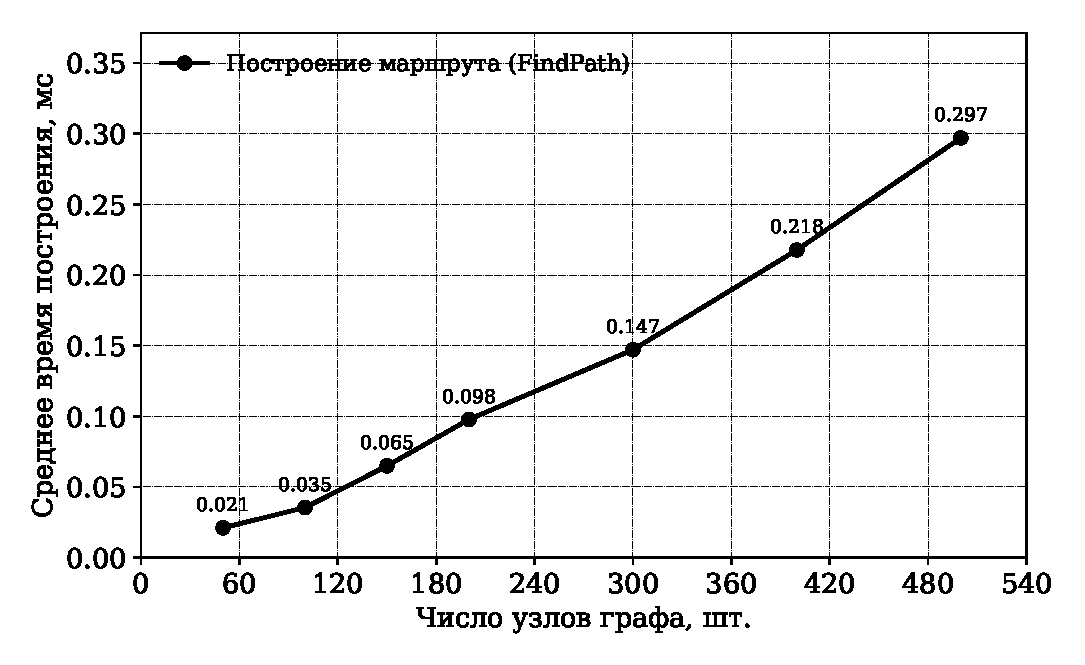
\includegraphics[width=0.85\textwidth]{Pictures/rpperf.eps}
\caption{Зависимость времени построения маршрута от размера графа}
\label{rpperf:image}
\end{figure}

Время выполнения растёт практически линейно с увеличением размера графа, что согласуется с теоретической оценкой сложности $O((V + E) \log V)$ для разреженных графов \cite{cormen}. Все измеренные значения находятся в субмиллисекундном диапазоне и укладываются в установленные требования с многократным запасом: даже на графе из 500~узлов построение маршрута занимает в среднем 0,297~мс при требовании менее 200~мс, а поиск ближайшего эвакуационного выхода -- 0,630~мс при требовании менее 300~мс. Полученный запас по производительности подтверждает пригодность алгоритма Дейкстры для построения маршрутов в реальном времени и оставляет резерв для графов значительно большего объёма.

\subsection{Системное тестирование}

Системное тестирование выполнено для проверки совместной работы всех компонентов приложения IndoorNav в сборе на реальных данных навигационного графа здания (586~узлов, 1202~ребра) и на целевых платформах (Windows, iOS, Android). В отличие от модульного тестирования, проверяющего отдельные методы, системное тестирование оценивает сквозные сценарии <<от действия пользователя до результата на экране>> с участием всех слоёв архитектуры -- представления, модели представления, сервисов и модели данных.

Ниже подробно описаны сквозные сценарии системного тестирования. Для каждого сценария приведены выполняемые действия и полученный результат, а для сценариев, проверенных в работающем приложении, -- снимок экрана.

\subsubsection{Построение маршрута между аудиториями}

\textbf{Сценарий.} Пользователь выбирает начальную и конечную аудитории и запускает построение маршрута на реальном графе здания. Система загружает граф, выполняет поиск кратчайшего пути алгоритмом Дейкстры и формирует пошаговые инструкции.

\textbf{Результат.} Построен кратчайший маршрут между аудиториями, отображён на плане этажа; сформированы пошаговые инструкции. Результат соответствует требованию построения маршрута между точками и показан на рисунке~\ref{rproute:image}.

\begin{figure}[H]
\centering
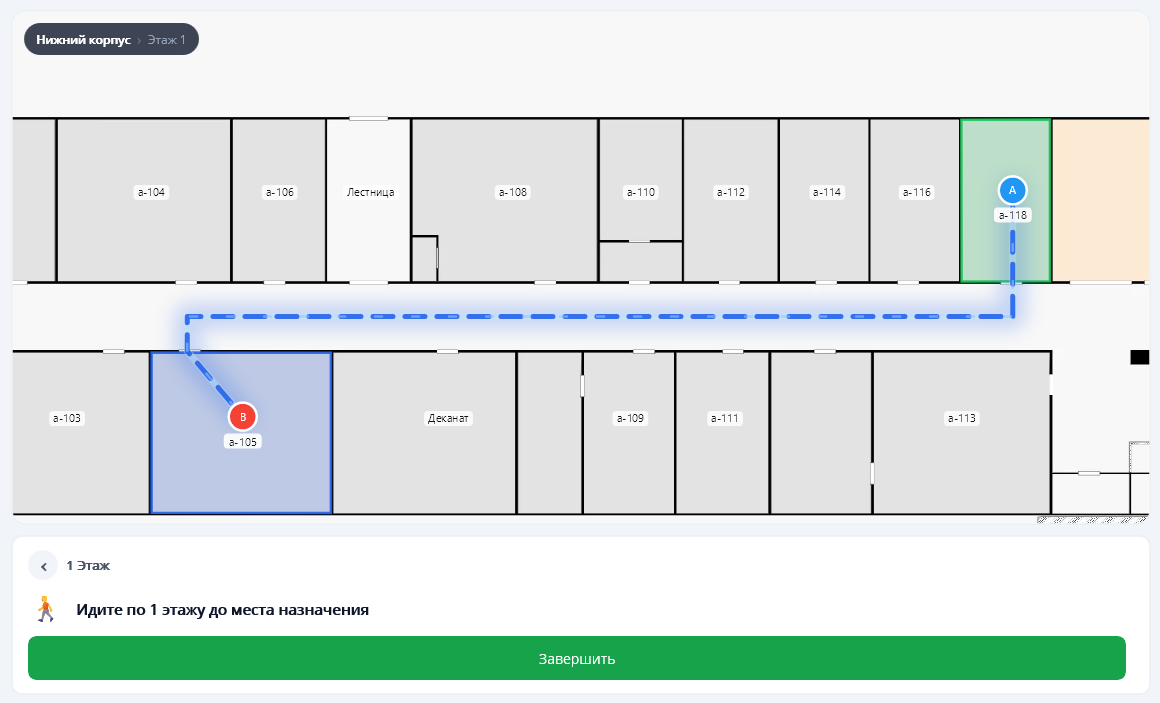
\includegraphics[width=0.95\textwidth]{Pictures/rproute.png}
\caption{Построение маршрута между аудиториями}
\label{rproute:image}
\end{figure}

\subsubsection{Эвакуационный маршрут в режиме ЧС}

\textbf{Сценарий.} Администратор активирует режим чрезвычайной ситуации, после чего система автоматически строит маршрут до ближайшего эвакуационного выхода от текущего положения пользователя.

\textbf{Результат.} Построен маршрут до ближайшего выхода. Результат соответствует требованию работы режима ЧС и показан на рисунке~\ref{rpemergency:image}.

\begin{figure}[H]
\centering
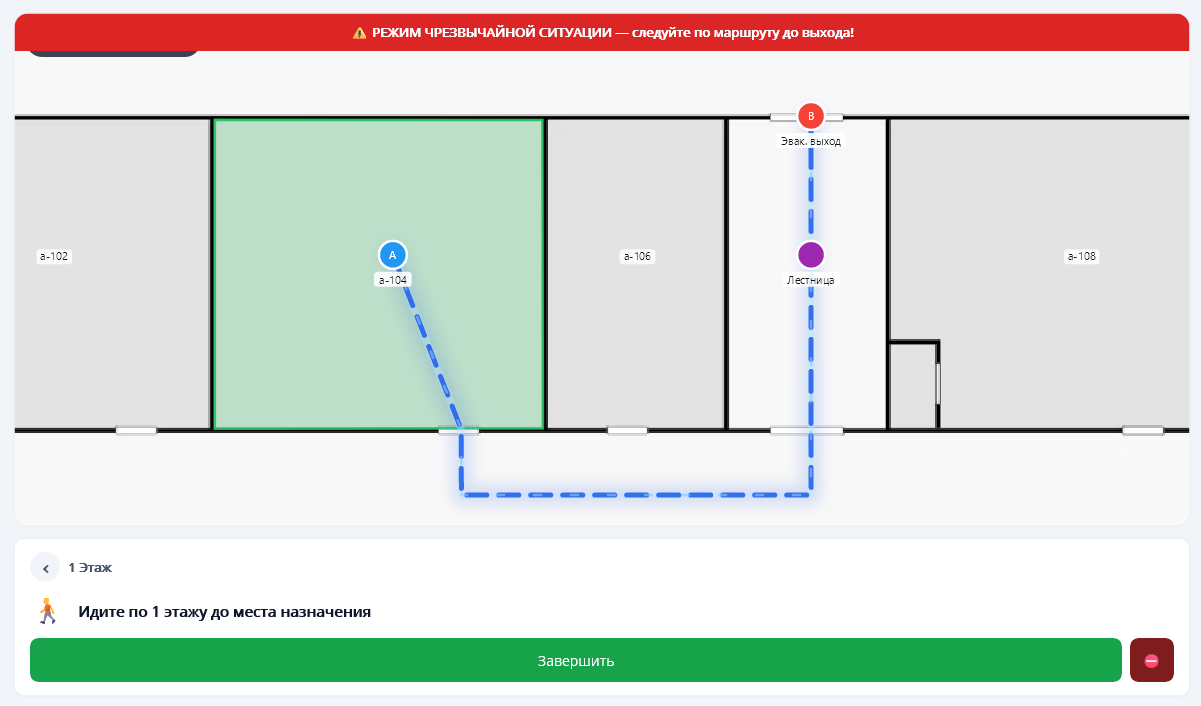
\includegraphics[width=0.95\textwidth]{Pictures/rpemergency.png}
\caption{Эвакуационный маршрут до ближайшего выхода в режиме ЧС}
\label{rpemergency:image}
\end{figure}

\subsubsection{Перестроение маршрута при блокировке}

\textbf{Сценарий.} Пользователь отмечает заблокированный узел на текущем маршруте, после чего система перестраивает путь.

\textbf{Результат.} Маршрут автоматически перестроен в обход заблокированного участка без перезагрузки графа. Результат подтверждает работу механизма динамического исключения узлов и показан на рисунке~\ref{rpreroute:image}.

\begin{figure}[H]
\centering
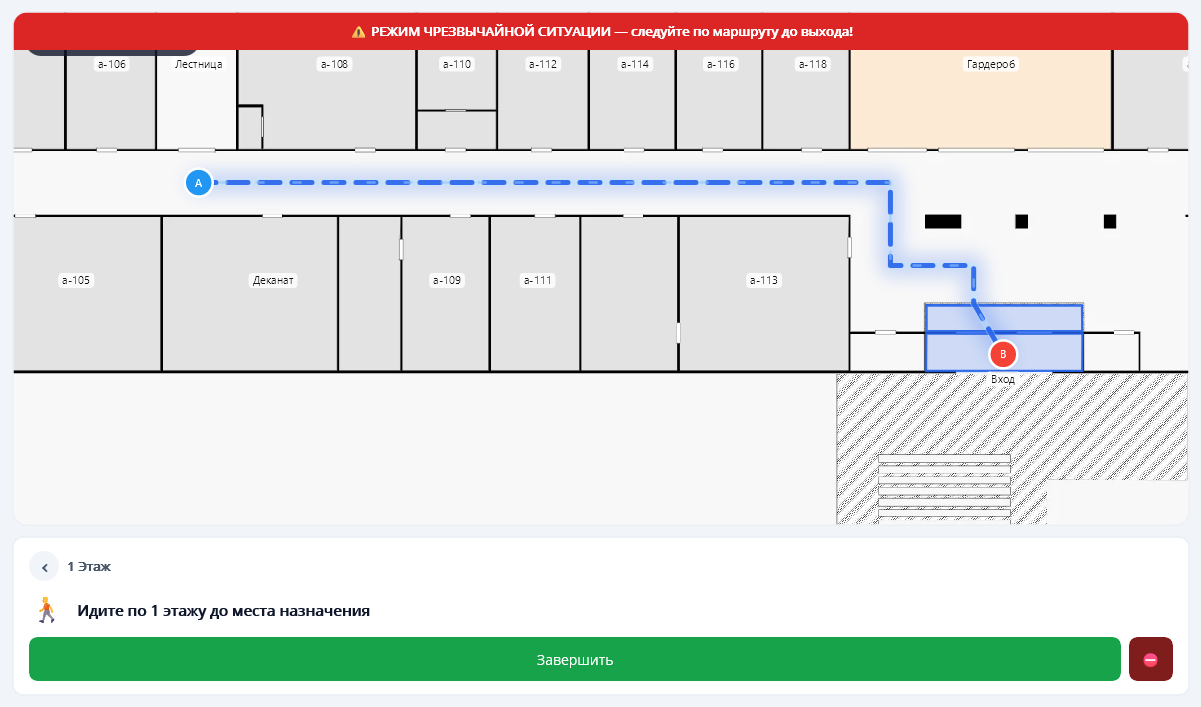
\includegraphics[width=0.95\textwidth]{Pictures/rpreroute.png}
\caption{Перестроение маршрута при блокировке участка}
\label{rpreroute:image}
\end{figure}

\subsubsection{Позиционирование пользователя по QR-коду}

\textbf{Сценарий.} Пользователь сканирует QR-код, размещённый на стене здания. Приложение разбирает ссылку вида \texttt{indoornav://node/\{id\}}, устанавливает соответствующий узел как начальную точку.

\textbf{Результат.} Начальная точка маршрута корректно определена по отсканированному QR-коду. Результат подтверждает интеграцию модуля разбора ссылок с алгоритмом маршрутизации и показан на рисунке~\ref{rpsys2:image}.

\begin{figure}[H]
	\centering
	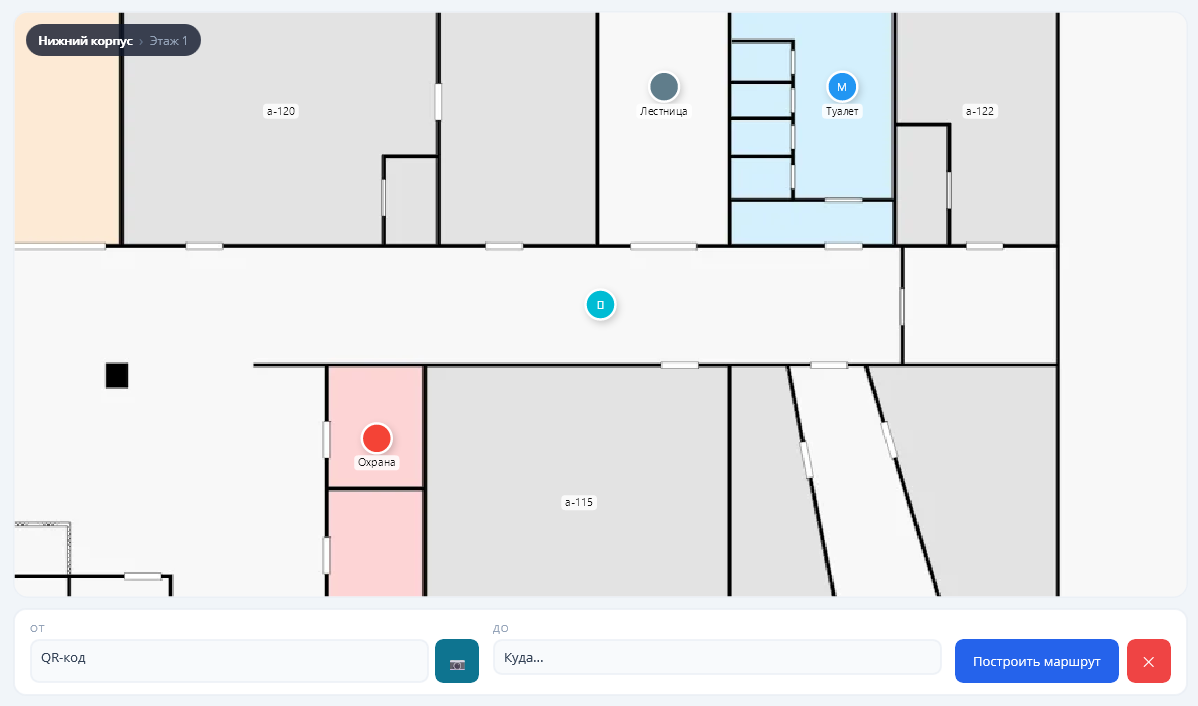
\includegraphics[width=0.95\textwidth]{Pictures/rpsys2.png}
	\caption{Позиционирование пользователя по QR-коду}
	\label{rpsys2:image}
\end{figure}

\subsubsection{Определение исходной точки по расписанию в режиме ЧС}

\textbf{Сценарий.} В здании активирован режим чрезвычайной ситуации. При входе студента в приложение система запрашивает подтверждение того, что он находится в аудитории согласно своему расписанию. При подтверждении эта аудитория автоматически устанавливается как исходная точка, и сразу строится маршрут до ближайшего эвакуационного выхода.

\textbf{Результат.} Исходная точка маршрута определена по подтверждённой аудитории из расписания без ручного выбора, эвакуационный маршрут до ближайшего выхода построен автоматически. Результат подтверждает совместную работу сервиса расписания и модуля эвакуационной маршрутизации и показан на рисунке~\ref{rpsys3:image}.

\begin{figure}[H]
	\centering
	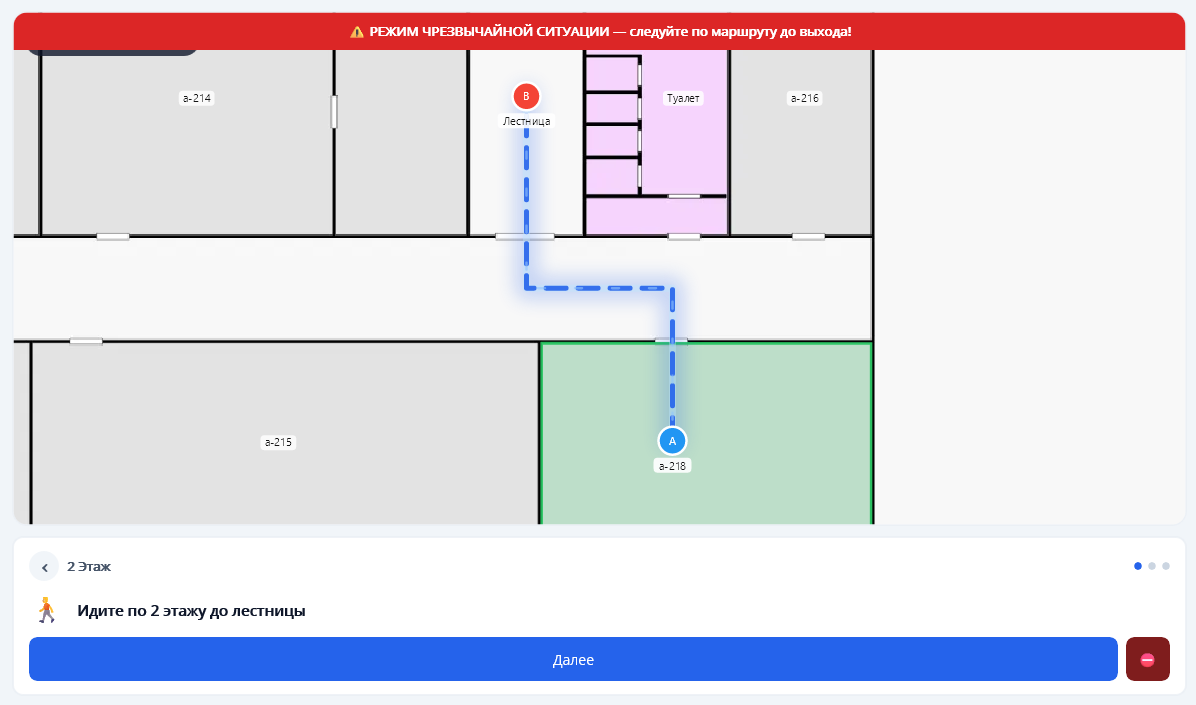
\includegraphics[width=0.95\textwidth]{Pictures/rpsys3.png}
	\caption{Определение исходной точки по расписанию в режиме ЧС}
	\label{rpsys3:image}
\end{figure}

Системное тестирование подтвердило корректную совместную работу всех слоёв приложения на реальных данных графа здания и на целевых платформах.

